\documentclass[journal]{IEEEtran}
\usepackage{times}

% numbers option provides compact numerical references in the text. 

\usepackage{graphics} % for pdf, bitmapped graphics files
\usepackage{epsfig} % for postscript graphics files
%\usepackage{mathptmx}
%\usepackage{newtxtext}
%\usepackage{newtxmath}
\usepackage{times} % assumes new font selection scheme installed
\usepackage{amsmath} % assumes amsmath package installed
\usepackage{amssymb}  % assumes amsmath package installed
\usepackage{amsthm}
\usepackage{mathtools}
\usepackage{bm}
\usepackage{mathrsfs}
\usepackage{xcolor}
\usepackage{cite}
\usepackage{threeparttable}
\usepackage{multirow}
\usepackage{bigdelim}
\usepackage{algorithm}
\usepackage{algorithmicx}
\usepackage{algpseudocode}
\usepackage{graphicx}
\usepackage{subfigure}
\usepackage{comment}
\usepackage{pifont}
\usepackage{mnsymbol}

\usepackage{amsmath}

\usepackage[numbers]{natbib}
\usepackage{multicol}
\usepackage[bookmarks=true]{hyperref}

\newtheorem{theorem}{Theorem}
\newtheorem{definition}[theorem]{Definition}
\newtheorem{lemma}[theorem]{Lemma}
\newtheorem{corollary}[theorem]{Corollary}
\newtheorem{proposition}[theorem]{Proposition}
\newtheorem{remark}[theorem]{Remark}

%\pdfinfo{
%  /Author (Homer Simpson)
%   /Title  (Robots: Our new overlords)
%  /CreationDate (D:20101201120000)
%   /Subject (Robots)
%   /Keywords (Robots;Overlords)
%}

\begin{document}

\title{An Improved Maximal Continuity Graph Solver for Non-repetitive Manipulator Coverage Path Planning}

\author{Tong Yang, Jaime Valls Miro, Yue Wang$^*$ and Rong Xiong
\thanks{$^1$ Tong Yang, Yue Wang and Rong Xiong are with the State Key 
Laboratory of Industrial Control and Technology, Zhejiang University, P.R. China. 
}
\thanks{$^2$ Jaime Valls Miro is with the Robotics Institute at the University of Technology Sydney (UTS:RI), Sydney, Australia.}
\thanks{$^*$ Corresponding Author. \newline \indent
E-mail address: {\tt\small wangyue@iipc.zju.edu.cn}}
}

\maketitle

\begin{abstract}
A provable computational improvement to the problem of maximal continuity during non-repetitive object coverage with non-redundant manipulators is proposed in this work, where the physical meaning of optimality translates to minimal number of end-effector lift-offs. Existing solutions enumerate each point on the surface with multiple ``colours'' according to the joint-configuration adopted, and model the problem as a painting problem of a graph with $M$ topological cells (a fully-connected section of end-effector points that can be painted with the same set of possible colours) and $N$ topological edges
(indicating the different choices of colour available). 
These works have proven that all optimal solutions can be collected in a finite number of steps. However, the solution grows exponentially in the size of $M, N$, becoming potentially intractable even for relatively simple graphs.
The proposed solution aims to avoid the need to enumerate all 
the edges by exploiting a topological invariance observed at colour intersections: 
the solution of an intersection-free graph can be uniquely represented by the colour of its boundary cells (in order), while enumerating internal edges and cells 
are shown to make no difference to the optimality of the solution, and can be safely omitted. 
A novel strategy is thus proposed to separate the graph into intersection-free sub-graphs.  
After enumerating and combining the solutions to each sub-graph to form the set of all optimal solutions, 
the complexity is proven to be reduced by a factor of $2^N$. Challenging scenarios are presented to validate the computational advantage of the proposed strategy.
\end{abstract}

\begin{IEEEkeywords}
Optimal Cellular Decomposition, Manipulator Coverage Task
\end{IEEEkeywords}

\IEEEpeerreviewmaketitle

\section{Introduction and Related Work}
\label{section_introduction}
The work in this manuscript is motivated by the non-revisiting coverage path planning (NCPP) along the surface of an object~\cite{Paul2013Novel}~\cite{Bhatt2019Concurrent} with a non-redundant manipulator, as illustrated by~Fig.~\ref{fig:toy_coverage_example}. 
Given the object's surface, the manipulator, 
the surrounding obstacles in the workcell and their related poses, for each reachable point on the surface there exist a finite number of inverse kinematic solutions in the manipulator configuration space, an example of which is depicted by the example mapping provided in~Fig.~\ref{fig:toy_coverage_graph_example}, left. 
Disregarding singular configurations~\cite{Yoshikawa1990Translational}, the collection of all valid configurations form disjoint sets in joint-space. When the manipulator transits from one set to another, it adopts a new pose altogether whereby the end-effector cannot remain on the object, being forcibly detached from the surface. This is an undesirable effect for tasks where smoothness and continuity are critical such as painting~\cite{li2011painting}, deburring~\cite{xie2016grinding}, welding~\cite{lee2011optimal}, scanning~\cite{Giataganas2013Cooperative} etc. 
In these instances, the desired solution translates to designing manipulator trajectories such that the end-effector visits each point on the surface exactly one time, whilst ensuring a minimum number of transitions between joint-space sets, or lift-offs. 

\begin{figure}[t]
\centering
\subfigure[Coverage illustration of a planar rectangular region with a non-redundant manipulator, depicting s(houlder)-l(eft)\&w(rist)-f(lipped), s-r(ight)\&w-u(nflipped), s-r\&w-f, and s-l\&w-u configurations. Transition between any pair imposes the adoption of a singular configuration thus preventing continuous traversability and a manipulator lift-off from the surface. By representing disconnectable manipulator configurations as different colours, an abstract topological graph % <JVM> I did not quite like the "task specificied" comment
with task-space colour distributions can be constructed as shown in (b) below.]{ % , the input to the NCPP problem. ]{
	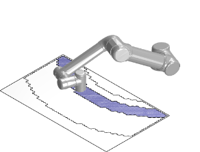
\includegraphics[width = 0.23\columnwidth]{figures/tmech_figures/slwf}
	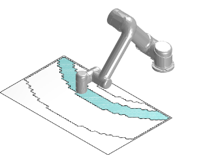
\includegraphics[width = 0.23\columnwidth]{figures/tmech_figures/srwu}
	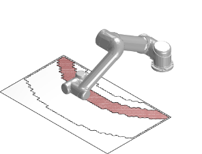
\includegraphics[width = 0.23\columnwidth]{figures/tmech_figures/srwf}
	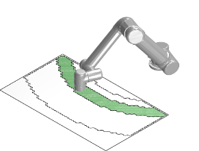
\includegraphics[width = 0.23\columnwidth]{figures/tmech_figures/slwu}
	\label{fig:toy_coverage_example}
}
\subfigure[Valid robot configurations form disjoint sets in joint-space, while their task-space FK mapping images (end-effector poses) may overlap. 
In the example, which for simplicity is illustrated with cells that are maximally $2$-overlapped, 
the resulting task-space graph conveys $N = 11$ undetermined edges constructed as shown by the dashed lines, thus separating the graph into $M = 11$ cells.
To facilitate the understanding whilst limiting clutter in the graph, 3 cells and 2 edges ($i$ and $j$ in dashed blue-green and blue-red respectively) are singled out. 
Solving the NCPP problem for the set of edges in the example can easily reveal all the optimal solutions in this case (two, depicted), demarcating the minimal bound for lift-offs as four. 
It is easy to appreciate how as more colours ``intersect", the algorithmic complexity to find the optimal solutions will soon escalate (more intricate examples are provided in Section~\ref{section_experiment}). It is also intuitive that should the green colour remain a complete set, both the red and blue colour cells would be split into further disconnected parts, 
leading to extra lift-offs. This hints at the fact ``intersecting" colours can be exploited to reduce the complexity of the solution.]{
	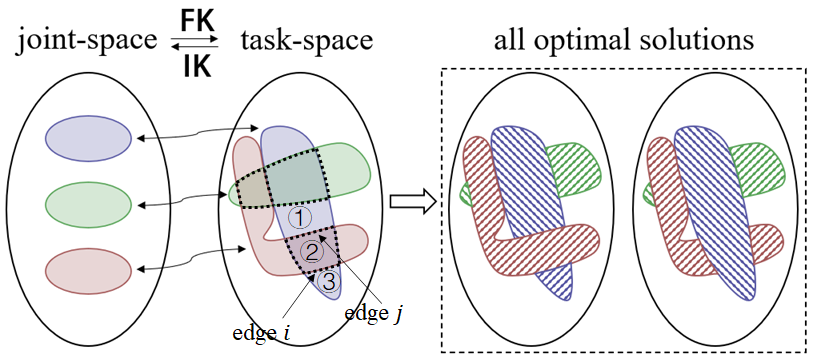
\includegraphics[width = 0.97\columnwidth]{figures/mapping_2}
	\label{fig:toy_coverage_graph_example}
}
\caption{A toy illustration of the problem arising when planning optimal non-revisiting coverage paths with a manipulator: (a) non-revisiting coverage of an object is dictated by the 
available configurations the manipulator can adopt. This leads to (b) disjoint sets in task-space, which conform the input to the NCPP problem. The optimal slicing of these sets leads to minimal discontinuities in tracing the surface with the end effector. (Please note the above separate examples are independently chosen to best illustrate the problem and do not correpond to each other).
}
\label{fig:mapping}
\end{figure}

\begin{comment}
\begin{figure}[t]
\centering
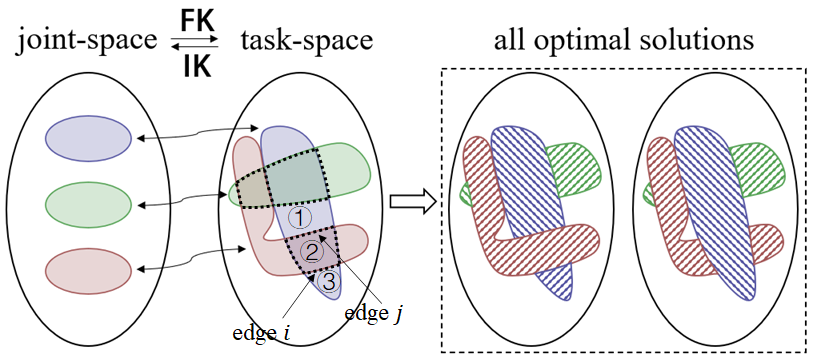
\includegraphics[width = 0.48\textwidth]{figures/mapping_2}
\caption{A toy illustration of the problem arising when planning optimal non-revisiting coverage paths with a manipulator: valid robot configurations form disjoint sets in joint-space, while their task-space FK mapping images (end-effector poses) may overlap. 
In the example, which for simplicity is illustrated with cells that are maximally $2$-overlapped, the resulting task-space graph conveys $N = 11$ undetermined edges constructed as shown by the dashed lines, thus separating the graph into $M = 11$ cells.
To facilitate the understanding whilst limiting clutter in the graph, 3 cells and 2 edges ($i$ and $j$ in dashed blue-green and blue-red respectively) are singled out.
Solving the NCPP problem for the set of edges in the example can easily reveal all the optimal solutions in this case (two, depicted), demarcating the minimal bound for lift-offs as four. 
It is easy to appreciate how as more colours ``intersect", the algorithmic complexity to find the optimal solutions will soon escalate (more intricate examples are provided in Section~\ref{section_experiment}). 
It is also intuitive that should the green colour remain a complete set, both the red and blue colour cells would be split into further disconnected parts, leading to extra lift-offs. 
This hints at the fact ``intersecting" colours can be exploited to reduce the complexity of the solution.
}
\label{fig:mapping}
\end{figure}
\end{comment}


Early reports on the generic \textit{coverage path planning} (CPP) problem focused on geometric path designing~\cite{Kaljaca2020Coverage}~\cite{Oriolo2005Motion}, particularly for mobile platforms operating in planar surfaces, such as boustrophedon~\cite{choset1998coverage} or spiral paths~\cite{hassan2018a}. 
Additional strategies were later proposed that transformed the coverable region into smaller partitions, or \textit{cells}, where continuous coverage paths could be guaranteed. A body of novel partitioning \textit{cellular decomposition} strategies emerged~\cite{Acar2002Morse}~\cite{choset2000exact}~\cite{huang2001optimal}~\cite{Atkar2009Hierarchical}~\cite{Hassan2017Simultaneous}, applied directly onto the area to be covered. This is an ineffective strategy when transferred from task to joint space for manipulator planning since the kinematic mapping between the two spaces is non-bijective: as illustrated in Fig.~\ref{fig:mapping}, the forward kinematic relationship from the configuration space to the surface is surjective (many-to-one) and locally flat (one-to-one from each connected component of the valid configuration space to the surface). 
The problem is further compounded when the end-effector can only visit each point on task-space once, leading to numerous pose reconfigurations during the motion of the end-effector~\cite{rososhansky2011coverage}.
Many criteria in the classic CPP problems have been adapted to the manipulator NCPP task, such as time to completion~\cite{lu2020time} or energy consumption~\cite{mei2004energy}, and optimal mobile manipulator pose for a given coverage in task-space has also been investigated~\cite{paus2017a}~\cite{Fan2021Base}~\cite{Kalawoun2018Optimal}. However, optimising  end-effector lift-offs for increased smoothness and continuity has been rarely exploited. 
Recent propositions in the literature to tackle the problem decomposed the task-space area into a topological graph ensuring continuous joint-space coverage within each cell, and looked for solutions where maximal continuity between cells existed~\cite{Yang2020Cellular}, as intuitively depicted in Fig.~\ref{fig:mapping}. 
All maximal-continuous cellular decompositions were proven to be collectable in a finite number of steps, defined by edges that represent the smallest, inseparable elements and cells that could only have a finite number of different sub-divisions.  

% <JVM> Content below ok, but not like this. I will change tomorrow, leave as is for now.
\begin{color}{blue}
\subsection{Preliminary and Complexity}
Given the kinematics of the non-redundant manipulator, the shape of the surface to be non-revisitably covered, the obstacles in the surrounding environment, and their related poses, each point on the surface can be reached by the end-effector through finite number of Inverse Kinematic (IK) solutions. Following topological elements are well-defined. 
\begin{definition}
(Valid Configuration) Valid configuration is the collision-free and non-singular~\cite{Yoshikawa1990Translational} manipulator configuration such that the end-effector touches the surface to be manipulated with its orientation parallel to the surface normal.  
\end{definition}
\begin{remark}
When singular configurations are disregarded, the FK relation from the manipulator configuration space to the space of end-effector poses is locally one-to-one.  
\end{remark}
\begin{definition}
(Colour) Each valid manipulator configuration is represented by a colour. Continuous configurations are assigned the same colour. Assume that there is an one-to-one correspondence between the EE pose and the point on the surface, the colour of a point on the surface represents the corresponding IK solutions with same colour. 
\end{definition}
\begin{definition}
(Cell) A cell is a maximal connected region on the surface, within which all points have the same number of valid IK configurations, and the configurations are pairwise continuous. 
In other words, all points have the same set of possible colours, which is also referred to as the possible colours of the cell. 
\end{definition}
\begin{remark}
By the definition of cell, within a single cell the geometric coverage path can be arbitrarily designed. 
And starting from any choice of configuration, the manipulator can continuously track the coverage path without end-effector lift-off. 
\end{remark}

\begin{definition}
(Edge) The edge is the common boundary of two cells.  
\end{definition}
\begin{definition}
(Graph) A graph is the combination of all cells and their connectivities, i.e., the edges. 
\end{definition}
Given the NCPP problem to be solved, the initial graph can be constructed. 
By saying \textit{solving the graph} we mean preserving only one of the possible colours for each point. 
During the solving process, if on the both side of the edge the points have the same possible colour, then it is equivalent to removing the edge. Or else it is equivalent to keeping the edge. 
Theoretical discussions~\cite{Yang2020Cellular} have be carried out to ensure that 
\begin{enumerate}
\item The number of cells in the initial topological graph is finite. 
\item The intersection of edges is isolated point, thus can be safely disregarded. 
\end{enumerate}
The following lemma has ensured the finiteness of all possible topological-distincted cellular decompositions, among which all optimal cellular decompositions lie in. 
\begin{lemma}\label{lemma:tmech_equiv}
(\cite{Yang2020Cellular}) Different part of a cell may be filled in different colours, while the design of the cell cutting paths satisfies that 
\begin{enumerate}
\item It is sufficient to consider cutting paths which start and end at the edge endpoints. 
\item It is unnecessary to consider cutting paths that go across edges.
\item It is unnecessary to consider intersecting cutting paths. 
\end{enumerate}
\end{lemma}
\end{color}

This is however an intensely computational process, growing exponentially in the size of the graph. Let there be $M$ topological cells and $N$ internal topological edges in the modelled graph to be solved. The number of edges for the $i$-th cell is $\alpha_i$, and denote the number of possible colours to fill cell $i$ as $K_i$.   
It has been shown how a binary array of length $\alpha_i$ can be used to index all possible different divisions of cell $i$~\cite{Yang2020Cellular}, whereby $0$ at a given position enforces the cell having a different color to its adjacent cell, whilst $1$ compels the same choice of colour. 
However, as supported by the illustrative example shown in Fig.~\ref{fig:many_to_one} for one of the edge solutions $(1111)$ and $2$ possible colours available for painting, the binary array does not uniquely represent a valid painting solution: the cell may be divided into two parts with differing colours, while each part themselves connect to their two adjacent cells. Following the cell sub-divisions, $4$ valid painting solutions of this cell appear corresponding to the edge solution $1111$. 

\begin{figure}[t]
\centering
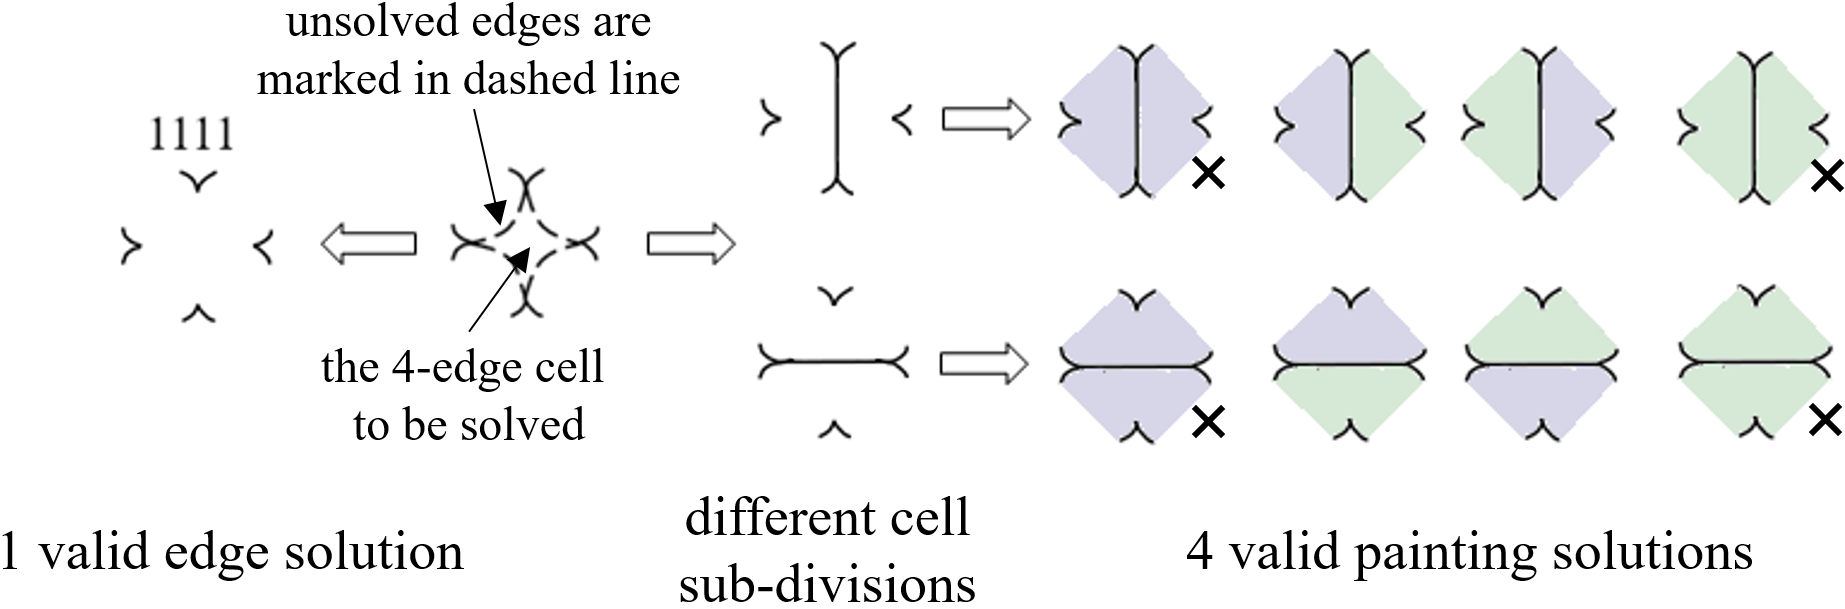
\includegraphics[width = 0.48\textwidth]{figures/many_to_one_3}
\caption{An illustration of the many-to-one relation between edge and painting solutions. 
Let a cell with $4$ adjacent cells (a $4$-edge cell) have 2 possible colours ``blue" and ``green", then $\alpha = 4, K = 2$. From the point of view of solving edges, the binary number $1111$ specifies one solution, but the corresponding valid painting solutions are multiple, $4$ to be precise: there are $E=2$ ways to divide the multi-edge cell into $3$-edge sub-cells, and $\alpha-2 = 2$ sub-cells are generated which can be filled with the $K (=2)$ possible colours. After enumerating $E\cdot K^{\max\{\alpha-2, 1\}}$ cases, four of them are removed (no subdivision when there is only one possible colour for all sub-cells), shown crossed-out, leaving the remaining four valid painting solutions.
}
\label{fig:many_to_one}
\end{figure}


\begin{comment}
Since every edge has two adjacent cells, 
the relation of $\alpha_i$ to $N$ is established by
\begin{equation}
N = \frac{1}{2}(\sum\limits_{i=1}^M \alpha_i - \tilde{N})
\end{equation}
($\tilde{N}$ simply denotes the number of edges on the outer boundary of the graph, %(with adjacent cells $-1$ ) 
which are determined and thus need not be enumerated). 
%Note that, although proving the finiteness of dividing each cell into sub-cells is enough for proving the finiteness of the whole process, the overall algorithmic complexity is far more than $2^N$, 
It has been shown in the Fig.~\ref{fig:many_to_one} counterexample how there is no one-to-one correspondence between the edge and painting solutions. 
The edge solution depicted, 1111, could be painted with 4 different valid painting alternatives.
Generically \textcolor{red}{is this from Tmech? I think so, so we need to reference it, not just drop it expecting the reader will be able to figure that out, not possible!} it has been proven by the cell sub-division strategy described in~~\cite{Yang2020Cellular} how if $\alpha_i \geq 4$, cell $i$ will be iteratively divided into $(\alpha_i-2)$ $3$-edge sub-cells\footnote{Here for simplicity we only consider the worst case presented in~\cite{Yang2020Cellular}. Beyond dividing fully into $3$-edge cells, the complexity of enumerating other cell sub-divisions is omitted \textcolor{red}{but it is also part of the enumeration of edges, shouldn't we? or you mean that taking the worst case, 4 adjacent cells, represents the highest computation and therefore we only need to consider this case for complexity calculation? - which I agree with}.}, and each sub-cell can be individually assigned with $K_i$ colours. Let there be $E_i$ different ways to divide cell $i$ into sub-cells, the overall complexity %\footnote{Here we disregard speeding-up tricks proposed in existing literature, because they are also valid in the algorithm proposed in this work. } 
can then be calculated as
\end{comment}

There is a need to enumerate all the edges for each cell, leading to all different colours to be subsequently filled in to create all posissible solutions~\cite{Yang2020Cellular}. This is a costly exercise. For the more generic case % we need this precision to figure out E_i
of a multi-edge ($\alpha_i \geq 4$) cell, other than the simple case of considering it as a whole, it may be sub-divided into up to $(\alpha_i-2)$ sub-cells, and each sub-cell can be individually assigned with $K_i$ colours. Considering a worst case scenario, let there be $E_i$ different ways to divide cell $i$ into $(\alpha_i-2)$ sub-cells, then $E_i\cdot K_i^{\max\{\alpha_i-2, 1\}}\cdot 2^{\alpha_i}$ steps are required for a single cell. Iteratively enumerating each cell and noting that each edge will only be enumerated once in the process, the algorithmic complexity can be calculated as
\begin{equation}\label{equ:tmech_complexity}
\prod\limits_{i=1\atop\alpha_i \geq 4}^{M}E_i\cdot \prod\limits_{i = 1}^M K_i^{\max\{\alpha_i-2, 1\}} \cdot 2^N
\end{equation}


\begin{comment}
Also note that as a dual graph of the commonsense ``node-edge" graph, the cells, edges and vertices correspond to the nodes, edges and faces (temporarily denoted as $F$ which has no usage in the NCPP problem), respectively. Then the relation of the number of cells $M$ and the edges $N$ is given by the Euler's formula for planar graph, 
\begin{equation}
N-M = F-2
\end{equation}
In a complicated graph we must have $F\gg 2$, then $N \gg M$. 
\begin{color}{blue}
We observe that enumerating an edge is a too trivial process to lead to different topologies of the resulting solution. See Fig.~\ref{fig:mapping}, where if edge $i$ is kept, then $j$ need not be removed, because even if cell \ding{172} and \ding{173} are connected, it makes no difference to the topology if cell \ding{174} is not connected together. 
In other words, existing works have avoided equivalent cellular decompositions under the equivalence of continuous modification of the cutting paths of cells. But looking at the topology of the resulting solution from a top-down view might further avoid carrying out equivalent multi-step processes in enumerative solving. 
In this paper, we introduce a high-level abstraction of the topology, the \textit{intersection}, which is the origin of the multiplicity of the optimal solutions. We show that intersections are unavoidable and have to be enumeratively solved. 
However, by separating the graph into intersection-free sub-graphs, all intersections are implicitly enumerated while sub-graphs are combined. As a result, the algorithmic complexity of enumerating all edges, $2^N$, is removed. 
\end{color}
\end{comment}


% <JVM> naming to be changed
\begin{color}{blue}
\subsection{Contribution of This Paper}
\end{color}

Careful examination of the topological graph leads in this work to the introduction of a high-level abstraction, the \textit{topologcal intersection} which is the origin of the multiplicity of the optimal solutions. It is hereby proven that intersections are indeed unavoidable and have to be enumeratively solved. However, separating the graph into intersection-free sub-graphs leads to all intersections being implicitly enumerated when the sub-graphs are recombined later to calculate the final solutions. The end result is the removal of the substantial complexity in enumerating all edges, $2^N$. 

\begin{figure}[t]
\centering
\subfigure[a cell-graph to be solved]{
	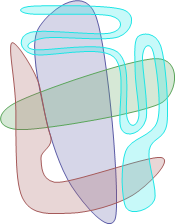
\includegraphics[width = 0.18\textwidth]{figures/cell_graph}
}
\subfigure[the node-graph]{
	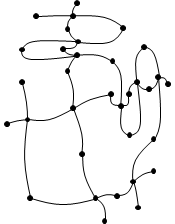
\includegraphics[width = 0.18\textwidth]{figures/node_graph}
}
\caption{The quantitive relation between the cell-graph adopted in manipulator coverage task and the node-graph discussed in classic graph theory. There are $33$ vertices, $39$ edges, and $8$ faces ($7$ cycles $+$ $1$ outer region reaching the infinity) in the node-graph, which correspond to $33$ cells and $39$ edges in the cell-graph. }\label{fig:node_graph}
\end{figure}

\begin{color}{blue}
The significance of the algorithmic improvement proposed in this work can also be revealed by mentioning the quantitive connection between the cell-graph utilised in manipulator NCPP task and the node-graph in classic graph theory, as shown in Fig.\ref{fig:node_graph}. There shall be an one-to-one correspondence between the cells and edges of a cell-graph and the vertices and edges in a node-graph, respectively, where then the Euler's formula~\cite{Bondy1976Graph} for planar graphs yields: 
\begin{equation}
V - E + F = 2
\end{equation}
where $V, E$ and $F$ are the number of vertices, edges and faces in the node-graph, respectively. This indicates the enormous number of edges in the cell-graph, $F-2$ greater than the number of cells, 
\begin{equation}
N - M = E - V = F - 2
\end{equation} 
Here it has been observed that in complicated graphs $F$ must be large, which acknowledges the contribution of reducing the algorithmic complexity by $1/2^N$. 
Also, the quantitive relation to the classic graph theory may indicate a potential application in other research areas besides the manipulator NCPP problem, which is beyond the scope of this work. 
\end{color}

The remainder of this paper is organised as follows. Section~\ref{section_intersection} introduces the concept of \textit{topological intersection} and the \textit{intersection-free graph} property.
Section~\ref{section_graph_separation} describes concrete steps to separate a graph into intersection-free sub-graphs. 
Solutions to these can then be combined to construct the optimal solutions for the full graph. 
Details about the complexity advantage in solving the problem following the proposed strategy is mathematically proven in Section~\ref{section_complexity}, whilst experimental results from simulations are collected in Section~\ref{section_experiment}. Final concluding remarks are gathered in Section~\ref{section_conclusion}.



\section{Optimality via ``Topological Intersections''}
\label{section_intersection}
In this section, we introduce a topological invariant variable, \textit{intersection}.  
%The enumeration of intersections will be shown to be the core element in the graph solver leading to notable inefficiencies in solving the full graph. 
\begin{color}{blue}
A topological invariant variable is a character of the given structure which is invariant under the admissible set of modifications to the structure, such as the connectedness of a region under homeomorphic mappings. 
Typical application of topological invariants in mathematics is for distinguishing two different objects: First define the topological invariant, then show that two objects have different topological invariants, so they are not equivalent under the modifications that preserve the topological invariant. 
However, different from the mainstream usage of topological invariants, we show that the enumerative solving of intersections is the core element in the graph solver leading to notable inefficiencies in solving the full graph. 
The key observation is then not leveraging intersections but how to avoid intersections. 

All contents in this sections are to contruct ``counterexamples" that reveal the inexistence of a possibly more efficient algorithm which avoids enumerating intersections. 
As will be concluded, the enumeration of all intersections, with their algorithmic complexity being multiplied, is unavoidable. 
Finally, all concentrations for possible improvement of the algorithmic complexity over existing algorithms have to be paid on avoiding ``explicitly" enumerating intersections, which makes the simplified representation of all solutions of an intersection-free graph apparent, and indicates an efficient algorithm based on intersection-free graph separation in the next section. 
%The simplified representation of all solutions of an intersection-free graph is then made apparent.  

\begin{figure}[t]
\centering
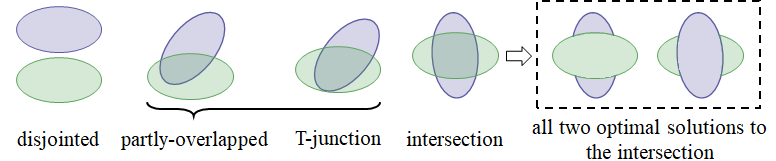
\includegraphics[width = 0.48\textwidth]{figures/basic_shape_3}
\caption{Illustration of basic relations between the reachable area of two colours. T-junction is a special case of the partly-overlapped distribution of colours, while it can be transformed back to a normal case through continuously modifying the boundary of colours. Only the intersected case needs solving, and it is apparent that the two optimal solutions are not topological equivalent, since they have the different number of connected regions in blue and green colour. }\label{fig:basic_shape}
\end{figure}


\begin{figure}[t]
\centering
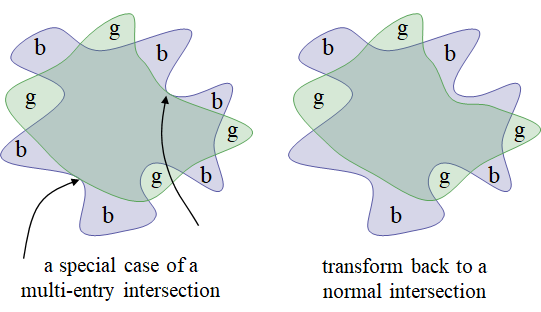
\includegraphics[width = 0.4\textwidth]{figures/multi_entry}
\caption{An intersection with $8$ entries. For some special cases that two consecutive adjacent cells can be filled in same colour, through shrinking the boundary of colour, it can be transformed back to the normal case. }\label{fig:multi_entry}
\end{figure}

\begin{figure*}[t]
\centering
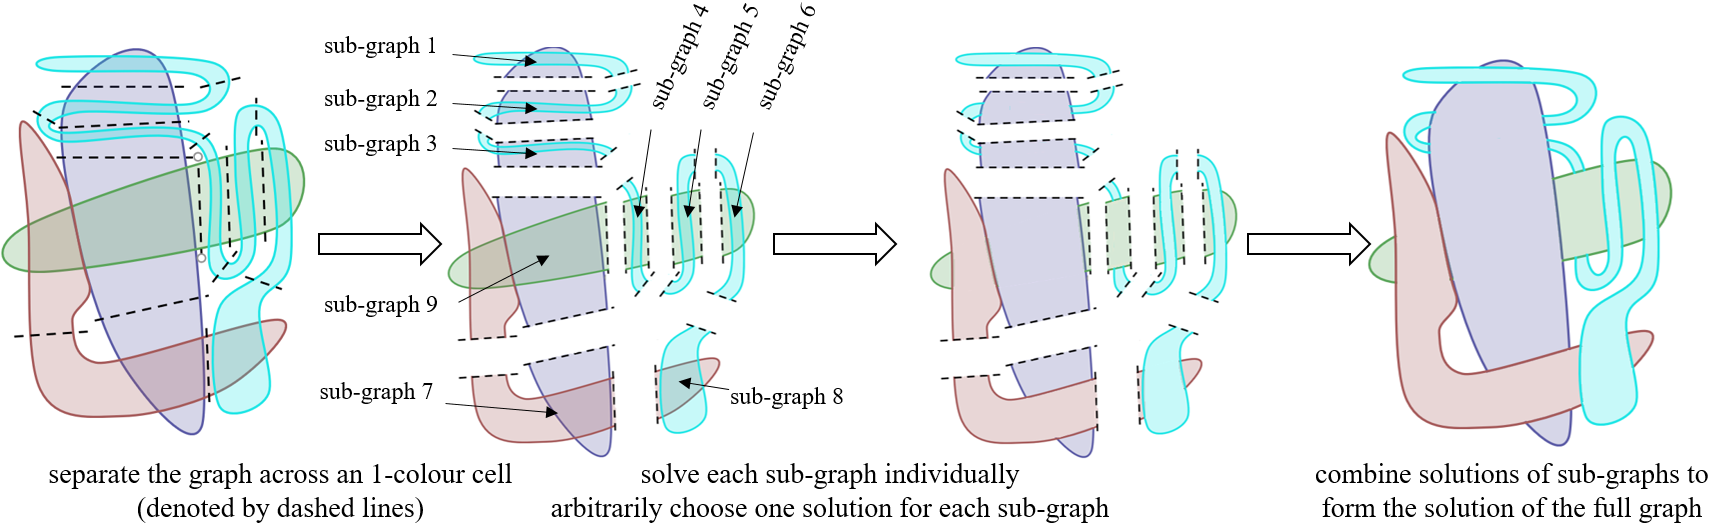
\includegraphics[width=\textwidth]{figures/two_overlapped_graph_2}
\caption{A maximally 2-overlapped graph to show the role of intersections. The full graph (left) is separated into $9$ sub-graphs through $1$-colour cells, shown with dashed cutting lines. Sub-graph $1$-$8$ has been shown to have two optimal solutions, while sub-graph $9$ gets a unique optimal solution after enumerative solving. Note that whatever solution gets chosen in each sub-graph, when two sub-graphs are combined, the two $1$-colour sub-cells separated by the dashed line re-join together, resulting in a reduction of one on the number of continuous regions. In total $4+(3\times 8)=28$ connected regions can be observed after solving the sub-graphs individually, combined with cost $-15$ (number of dashed lines). The nonrepetitive coverage problem of this graph ends up with $28-15=13$ connected regions, i.e., $12$ lift-offs. 
Note that no intersections in the full graph are avoided when solving all the sub-graphs. And different choices of the solution for each sub-graph will double the number of optimal solutions of the full graph: there will be $2^8=256$ optimal solutions to the graph.
}
%The number of continuous regions is $4+(3\times 8) = 28$  \textcolor{red}{??}, and $15$ dashed lines are created  \textcolor{red}{why? you say what you do, not why?}, so the number of continuous regions in the original graph is $28-15=13$, i.e., $12$ lift-offs are necessary to finish this coverage task. However, for all optimal cellular decompositions, each intersection has to be enumerated. The total number of optimal cellular decompositions will be $2^8 = 256$ \textcolor{red}{why?}, and no two of them are equivalent under continuous modification of cell boundaries \textcolor{red}{is this apparent in the figure? I can't see it}. 
\label{fig:two_overlapped_graph}
\end{figure*}


\subsection{Defining Intersections}
\begin{definition}
(Intersections) An intersection is a class of distribution, more concretely, overlapping, of the coverable region of multiple colours, describing an inevitable interruption of the connectedness of one colour 
by other colours. 
\end{definition}
Denoting $\#\{\mbox{NCPP}(G)\}$ as the minimal number of end-effector lift-offs given the graph $G$, and $\#\{\mbox{CPP}(G)\}$ as that of the repetitive coverage path planning problem, the existence of intersections can be formally revealed by
\begin{equation}
\mbox{intersection exists}\Leftrightarrow \#\{\mbox{NCPP}(G)\} - \#\{\mbox{CPP}(G)\} > 0
\end{equation} 
The invariance of intersections is revealed in the connectedness of cells: 

\begin{proposition}\label{lemma:invariance}
(Invariance under homotopic cutting paths) In a (partly-solved) graph, any continuous modification of the cell cutting paths will not reduce the number of intersections in the graph. 
\end{proposition}
\begin{proof}
It has been shown in \textbf{Lemma}~\ref{lemma:tmech_equiv} that all cutting paths (and preserved edges) need not to be intersected, hence the continuous modification of cutting paths will not change the connectivity of any cell. I.e., there will not be a case that two disconnected cells with the same colour filled become connected after continuous modification of cutting paths, nor a case that a single solved cell is trancated into two disconnected parts. Hence the intersections will be invariant. 
%There is certainty in the fact that the number of intersections in a partly-solved graph will not reduce under continuous modification of cell cutting paths. 
\end{proof}

Typically, for the simplest case, the coverable area of two colours may be fully disjointed, partly overlapped or intersected, as shown in Fig.~\ref{fig:basic_shape}, 
whereby colours can be both kept connected in the disjointed and partly overlapped cases, but critically in the intersection case one colour being connected will truncate the other colour into two parts.

 

\subsection{Properties of Intersections}
Each result in this subsection presents a crucial property of intersection. These properties are ``traps" that prevent an efficient algorithm being proposed. 
Note that they do not directly contribute to the algorithm design, but as a side effect indicate the possible upper bound of the improvement on the algorithmic complexity. 


\begin{lemma}
(Multiplicity of Solutions) The existence of intersections causes multiplicity of optimal NCPP solutions. 
\end{lemma}
\begin{proof}
For the most apparent example see Fig.~\ref{fig:basic_shape}. Obviously, there are two optimal solutions to the intersected case, filling in the central cell full of either blue or green. 
In more complicated graphs, such an intersection may introduce two sets of optimal solutions, in one set all solutions keep the blue colour connected, 
while in the other set the green colour remains connected. 

Note that the example is simple but not a special case. Assume that except one intersection, the left-out graph has been solved and $m$ solutions have been constructed, labelled as $s_1, \cdots, s_m$. Let there be $n$ different solutions of an intersection labelled by $t_1, \cdots, t_n$, then $m\times n$ solutions for the whole graph are constructed. 
Should the solution $(s_i, t_j)$ be (non-)optimal, $(s_i, t_{j'}), \forall j'\in \{1, \cdots, n\}$ would be also (non-)optimal. 
\end{proof}


\begin{corollary}
(Unavoidability of Enumeration) All intersections have to be enumerated in order to collect all optimal NCPP solutions. 
\end{corollary}

We prove this by showing two aspects:  
\begin{enumerate}
\item Collecting all solutions of a single intersection requires enumeration. 
\item Each intersection will not be removed by graph separation. Thus it can only be reduced by (enumerative) solving. 
\end{enumerate}
\end{color}

\begin{proof}
\begin{color}{blue}
1) We prove by example that even a kind of simple intersections, the multi-entry intersections, which are so structural to be easily solved, have to undergo an enumerative solving. 
\end{color}
Seeing the intersection in Fig.~\ref{fig:basic_shape} as $4$ entries, the intersection with arbitrary number of entries is intuitive, as shown in Fig.~\ref{fig:multi_entry}. 
After simplifying the case by merging consecutive adjacent cells which have the same set of possible colours, the intersection will have $n$ (an even number) entries. 
It is observed that for each adjacent cell (say the $i$-th, labelled cyclicly), if it is connected to any other adjacent cell through the intersection, then another two entries, $(i-1)$ and $(i+1)$, cannot be connected. So the minimal number of connected regions for an $n$-entry intersection is $\frac{n}{2}+1$. 
However, note that even if the optimal number is directly deduced, we still have to enumeratively solving the intersection to get all optimal cellular decompositions. 
For the $i$-th entry, we will separately consider (a) connecting it to other entries, or (b) keeping itself disconnected so that entries $(i-1)$ and $(i+1)$ can be connected. Both of them go to optimal cellular decompositions. 

2) The role of intersections in graphs can be revealed in solving a kind of simple graphs, separable maximally $2$-overlapped graphs, 
illustrated by Fig.~\ref{fig:two_overlapped_graph}.  
The key step is to separate the graph into sub-graphs by dividing $1$-colour cells connecting intersections. 
Since the divided cell only has a unique coverable colour, we divide one cell into two unconnectable cells (they belong to different sub-graphs), so the number of continuous regions on the graph should be the sum of continuous regions in sub-graphs minus the number of dashed lines. 
Moreover, we can arbitrarily combine the optimal solutions of sub-graphs to form the optimal solution of the original graph. 
However, it should be noted that while the computational cost of combining solutions of sub-graphs has been reduced, no intersection was removed. 
Intersections must be solved within the sub-graphs, and all optimal solutions collected through a full combination of the different solutions with 
intersections. %, as further described in Section~\ref{section_full_graph}.
\end{proof}

All above results have been proved by raising example graphs where the intersections can be easily distinguished. However, this is only for simple explanation, as in generic graphs the necessity of enumerative solving is compounded by the incountability of intersections. 

\begin{figure}[t]
\centering
\subfigure[The graph is observed to have $1$ intersection. ]{
	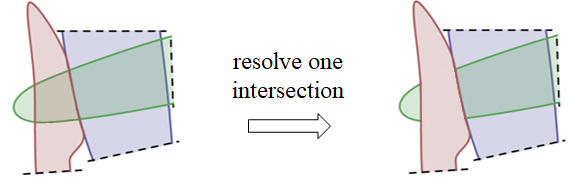
\includegraphics[width=0.4\textwidth]{figures/add_1}
}
\subfigure[Two intersection-free graphs form a graph with one intersection. ]{
	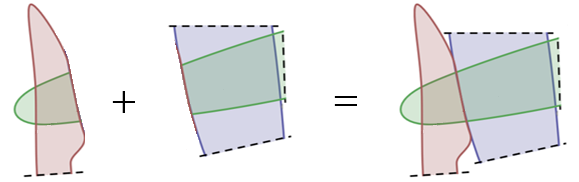
\includegraphics[width=0.4\textwidth]{figures/add_2}
}
\subfigure[After removing one intersection, the left-out part of an intersection-one graph still has one intersection. ]{
	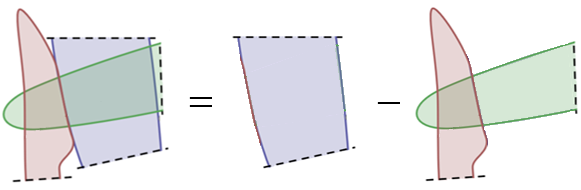
\includegraphics[width=0.4\textwidth]{figures/add_3}
}
\caption{The $0 + 0 = 1$ and $1 - 1 = 1$ example of the number of intersections between graph and sub-graphs. }\label{fig:add}
\end{figure}

\begin{color}{blue}
\begin{lemma}
(Incountability of Intersections) Given a graph, except the trivial cases, $0$ adn $1$, the number of intersections in the graph is not countable. 
\end{lemma}
\end{color}
\begin{proof}
Fig.~\ref{fig:two_overlapped_graph} sub-graph $9$ illustrates the case where two parallel (nonoverlapping but touching) colour regions exist which are simultaneously crossed by a third colour. In this case, the graph cannot be trivially separated since the multi-colour cells are adjacent, with no $1$-colour cell in between. 

\begin{color}{blue}
Analysing the sub-graph $9$ in detail gives us surprising results, as shown in Fig.~\ref{fig:add}. 
It can be easily observed that the graph has only one intersection, as after the intersection between red colour and green colour is resolved, the graph will have no intersection. 
However, a combination of intersection-free graph can generate an intersection-one graph, namely $0+0 = 1$ (Fig.~\ref{fig:add}(b)). 
From another perspective, after the blue colour is removed which apparently has an intersection with the green colour, the left-out graph still has an intersection, namely $1-1 = 1$ (Fig.~\ref{fig:add}(c)). 
\end{color}

In generalised cases encountered as shown in Fig.~\ref{fig:three_overlapped_graph}, it is apparent how as more colours get involved, intersections become highly coupled, and even identifying intersections is not trivial. 
\end{proof}

\begin{color}{blue}
\begin{corollary}
There is no algorithm that can solve a graph with explicit intersection-decreasing, such as transforming an intersection-$n$ graph to an intersection-$(n-1)$ partly-solved graph.
\end{corollary}

It can be thus concluded that all solvers (including all existing solvers and ours to be proposed in this work) to this problem have to be in an enumerative scheme, and there is no guarantee of the decreasing of the number of intersections as a graph being gradually solved. Only what we know is that a solved graph has no intersection. 
\end{color}
Disregarding the position of intersections and how to solve them leads to exhaustive implicit enumeration when all edges and cells are enumerated~\cite{Yang2020Cellular}. 
On the other hand, exploiting the interesting complex scenarios that analysing the topology between different colours offer will attenuate this problem. In this regard, the concept of intersection-free graphs described next will play a crucial role.  

\begin{figure}[t]
\centering
%\subfigure[]{
%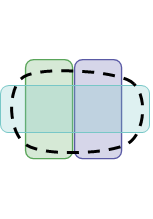
\includegraphics[height=0.06\textwidth]{figures/1_2_intersection}
%}
\subfigure[]{
	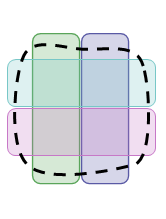
\includegraphics[height=0.07\textwidth]{figures/2_2_intersection}
}
\subfigure[]{
	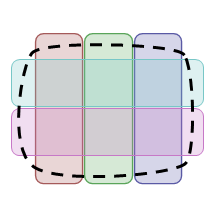
\includegraphics[height=0.07\textwidth]{figures/2_3_intersection}
}
\subfigure[]{
	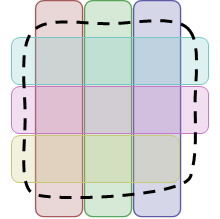
\includegraphics[height=0.07\textwidth]{figures/3_3_intersection}
}
\subfigure[]{
	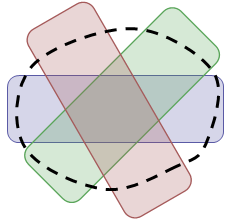
\includegraphics[height=0.07\textwidth]{figures/3_intersection}
}
\subfigure[]{
	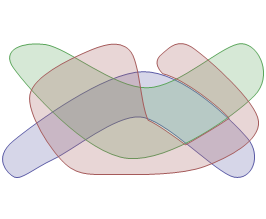
\includegraphics[height=0.07\textwidth]{figures/3_intersection_2}
}
\caption{Demonstrating graphs with various forms of intersections. 
The dashed circle marks a part of the graph which contains intersections. 
Intersection formed by: (a) $2\&2$ parallel colours, (b) $2\&3$ parallel colours and (c) a further special case of $3\&3$ parallel colours (where whether the orange colour intersects with the blue colour is closely related to the optimal solutions. Now they only form a T-junction), (d) a normal $3$-overlapped intersections and (e) a complicated $3$-overlapped graph which we cannot even figure out where is the intersection given too many intersections and parallels of colours in it. }\label{fig:three_overlapped_graph}
\end{figure}

\begin{figure*}[t]
\centering
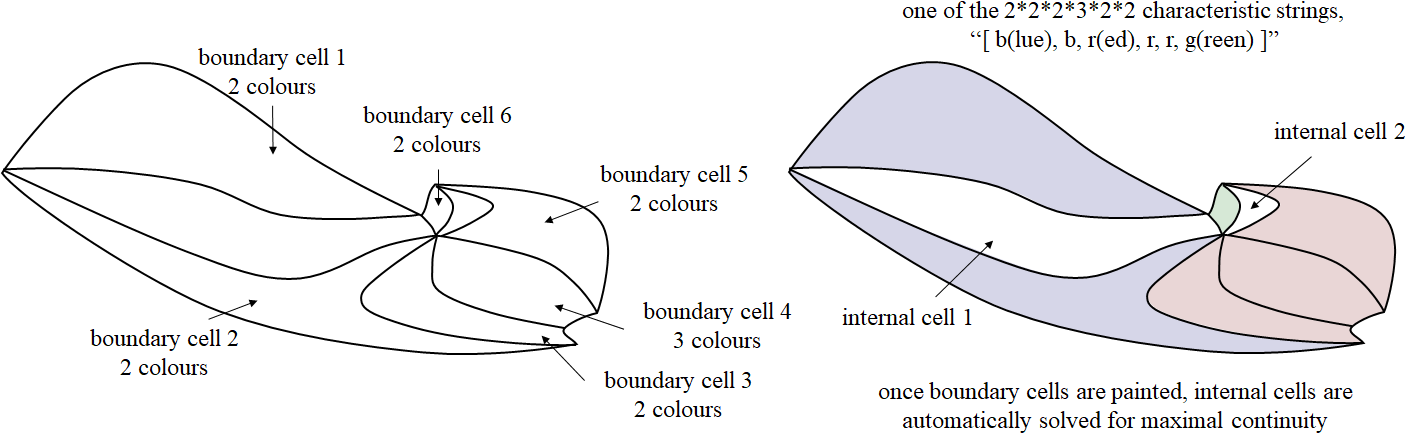
\includegraphics[width=0.9\textwidth]{figures/characteristic_string_2}
\caption{An intersection-free graph. The internal cell $1$ will choose blue $>$ green $>$ other colours. The internal cell $2$ will choose green $=$ red $>$ other colours.}\label{fig:characteristic_string}
\end{figure*}

\subsection{Intersection-Free Graphs}
\begin{definition}
(Intersection-free Graph) An intersection-free graph is a graph where no intersection can be constructed within it. 

(Boundary Cell, Internal Cell) Two types of cells can be distinguished in an intersection-free graph, the \textit{boundary cell} which has edges forming the boundary of the graph, and the remaining \textit{internal cell} which has no edge exposed to the graph boundary. 
\end{definition}
See Fig.~\ref{fig:characteristic_string} for an illustration of the intersection-free graph with $6$ boundary cells and $2$ internal cells. 
It is apparent that all internal cells are shown to have less than $4$ cells, or else an intersection could be constructed within. 

\begin{color}{blue}
\begin{definition}
(Characteristic String) Given a graph, let there be $n$ (ordered) boundary edges, then the characteristic string of the graph is a word of length $n$, where the $i$-th letter in the word represents the colour of the boundary cell containing the $i$-th boundary edge. 
\end{definition}

For the example in Fig.~\ref{fig:characteristic_string}, the partly painted graph has characteristic string ``[b, b, r, r, r, g]". 
\end{color}
A crucial property of intersection-free graphs is presented as the following theorem.
\begin{color}{blue}
\begin{theorem}
The solution of the graph, more concretely, the assigned colour of all cells in the graph, can be uniquely characterised by the colour of the boundary cells. 
\end{theorem}
\end{color}
\begin{proof}
To prove this, let the colour of all boundary cells be determined. On picking up two boundary cells with the same colour one must be able to judge their connectivity through this graph. Should connectivity be undetermined, one may find another pair of boundary cells whose connection may prevent these two cells being connected. However, this represents an intersection, which contradicts the assumption of intersection-free property of the graph. 

%The colour of the (ordered) boundary cells can be recorded in a string with length equalling the number of boundary edges of the graph, referred to as 
%the \textit{characteristic string} of the graph. 
After assigning a colour to each boundary cell, all internal cells will be assigned the colour which maximises the connectivity to their adjacent cells. 
After all cells have had their colour allocated, all the internal edges can be  automatically solved. 
It can thus be said that each characteristic string uniquely corresponds to a solution of the intersection-free graph, 
and the number of characteristic strings can then be liken to the full quantification of the number of solutions in the graph. 
\end{proof}
\begin{figure}[t]
\centering
\subfigure[]{
	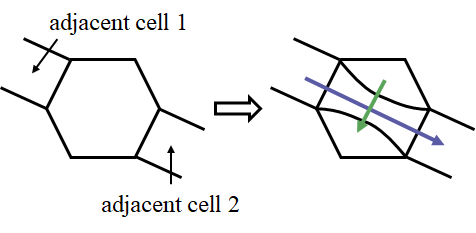
\includegraphics[width=0.22\textwidth]{figures/constraint_violation_a_2}
}
\subfigure[]{
	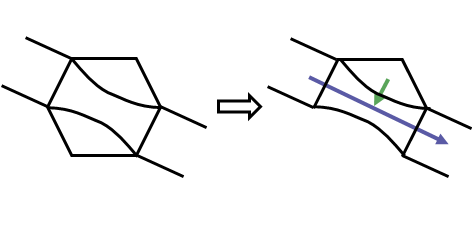
\includegraphics[width=0.22\textwidth]{figures/constraint_violation_b_2}
}
\caption{(a) Illustration of constraint violation due to cell sub-divisions in sub-graphs. One sub-cell will have four adjacent cells. (b) If a cell is scheduled to be divided, it should first be divided and the followed by constructing the intersection-free sub-graphs.}
\label{fig:constraint_violation}
\end{figure}

\section{Graph Separation}
\label{section_graph_separation}
%This motivates us to find a novel topological structure called \textit{width-$2$ strip}, or \textit{strip}, which is proven intersection-free. 
%With the graph being separated into strips and each strip being solved individually, we combine all solutions of strips to generate all solutions of the original graph, where all optimal solutions are included. 
%\textcolor{blue}{We might put this sentence to conclusion of this section: 
%Recall that intersections are intrinsic to the graph, non-existence of intersections in strips means that all intersections are automatically solved while strips are combined, which do not add extra algorithmic complexity. 
%}
 An efficient strategy to separate a graph into intersection-free sub-graphs is described in this section. 
Since non-adjacency of internal cells in sub-graphs will be enforced, and cell sub-divisions after sub-graphs have already been constructed, 
this constraint may be violated (see Fig.~\ref{fig:constraint_violation} for an illustration of this scenario).
So let at this point all $n(\geq 4)$-edge cells have been properly divided before applying the algorithm, 
thus all cells in the sub-graphs can only be seen as a whole and be filled with the same colour. 


An apparent result for graph separation is that the graph should not be separated across edges, or else the constraints of the original cell vanishes, and non-optimal solutions may appear. See an illustration of this scenario in Fig~\ref{fig:separation_at_edges}. 
Another result is that the optimality of part of the graph has no relation to the global optimal solution of the whole graph. 
This is proved by the example illustrated in Fig~\ref{fig:local_combined}. 

\begin{color}{blue}
An algorithm block showing the processes of intersection-free graph separation is given in \textbf{Algorithm} \ref{alg:1}. 

\begin{figure}[t]
\centering
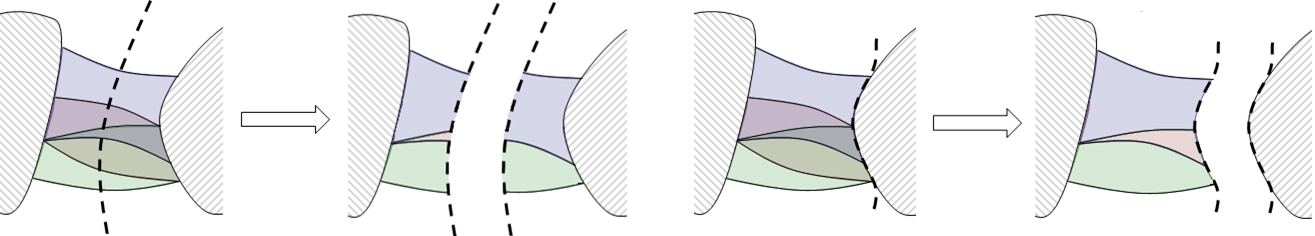
\includegraphics[width=0.48\textwidth]{figures/separation_at_edges_2}
\caption{If a graph is separated through division of multi-colour cells, the constraint of the cell vanishes, then in the sub-graphs there may exist solutions that after being combined is non-optimal, such as the case given in left. If the graph is separated along edges, we will not incur such problem. }\label{fig:separation_at_edges}
\end{figure}


%\subsection{Relation between Optimality of Graph and Its Sub-Graphs}
%Before we go into relations between graph and sub-graphs, we have to claim a basic criteria for separating a graph into sub-graphs. 
%Different from separating the graph through an $1$-colour cell, where the solutions of sub-graphs can be arbitrarily combined, if we separate the graph through multi-colour cells, as illustrated in Fig.~\ref{fig:separation_at_edges}, the constraints of the original cell vanishes, then proven non-optimal solutions may appear. In contrast, separating the graph through existing edges has the same effort, which is desired. 
%So in sequel our graph separation process should  follow existing edges in the graph, which makes Fig.~\ref{fig:non_optimal_subgraph} and Fig.~\ref{fig:local_in_other_graph} reasonable. 

%It is also observed that if the edge has multi-colour adjacent cells, then the combination of different solutions of sub-graphs will have non-trivial cost variation (not $-1$ as used in Fig.~\ref{fig:two_overlapped_graph}). 

\begin{figure}[t]
\centering
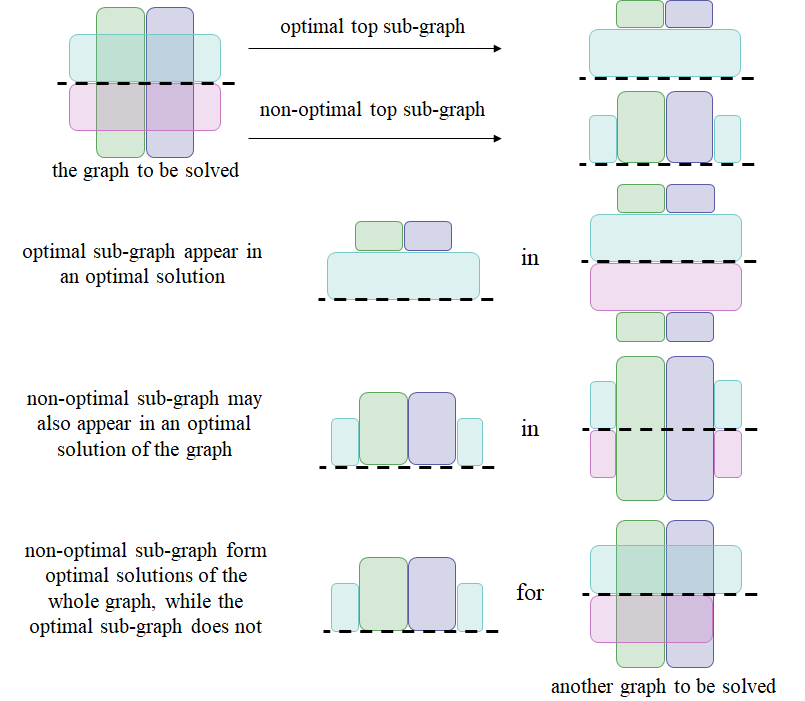
\includegraphics[width=0.48\textwidth]{figures/local_combined}
\caption{Separating the graph through the dashed line, we show the optimal solution and a non-optimal solution of the sub-graph. It is noticeable that both of them form optimal solutions of the original graph. An in the bottom case, as a sub-graph of another graph, the non-optimal sub-graph can form optimal solutions while the optimal sub-graph cannot do so. }\label{fig:local_combined}
\end{figure}

%Then, we claim that there is no guarantee about the global optimality of combining optimal solutions of sub-graphs. In other words, when a graph is separated into sub-graphs, we have to collect all solutions of each sub-graph. (It is not a bad thing if all solutions of sub-graphs can be enumerated, since in this case solving sub-graphs is unnecessary. )
%This is proved by two examples illustrated in Fig.~\ref{fig:non_optimal_subgraph} and Fig.\ref{fig:local_in_other_graph}. In \ref{fig:non_optimal_subgraph} both optimal and non-optimal solution of the sub-graph will form an optimal solution of the original graph. And in Fig.\ref{fig:local_in_other_graph} it is shown that non-optimal sub-graph is included in optimal solution of the original graph while the optimal sub-graph is not. 
%See Fig.\ref{fig:non_optimal_subgraph}, where the graph to be solved is an intersection between three parallel colours and another three parallel colours. The optimal solution is obviously either connecting all horizontal colours or connecting all vertical colours. 
%We can see from this case that optimality of the sub-graph is not equivalent to the optimality of the whole graph. So if a graph is separated into sub-graphs, we should store all solutions of sub-graphs but not only optimal solutions. 
%Another problem is that the optimality of a solution of the sub-graph hugely depends on other sub-graphs. A case is given in Fig.\ref{fig:local_in_other_graph}. 
%So we can only judge the optimality after we pick one solution from each sub-graph and combine them to form a solution of the whole graph. 
%In other words, in the absense of arbitrary combination of the solutions of sub-graphs, the algorithmic complexity of the graph is the multiplication but not the sum of the complexity of solving each sub-graph. 

\begin{figure*}[t]
\centering
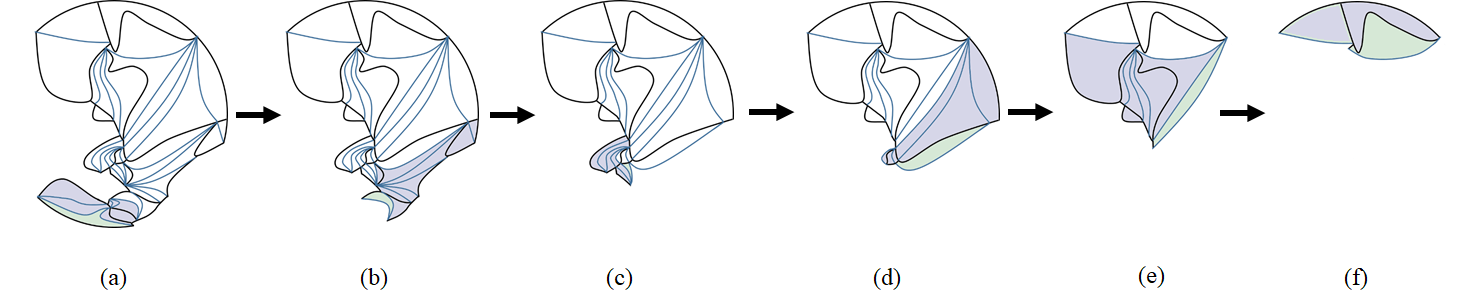
\includegraphics[width=0.96\textwidth]{figures/steps_2}
\caption{The concrete steps to separate the graph given in Fig.~\ref{fig:complicated_graph} into intersection-free strips. }\label{fig:steps}
\end{figure*}

\begin{figure*}[t]
\centering
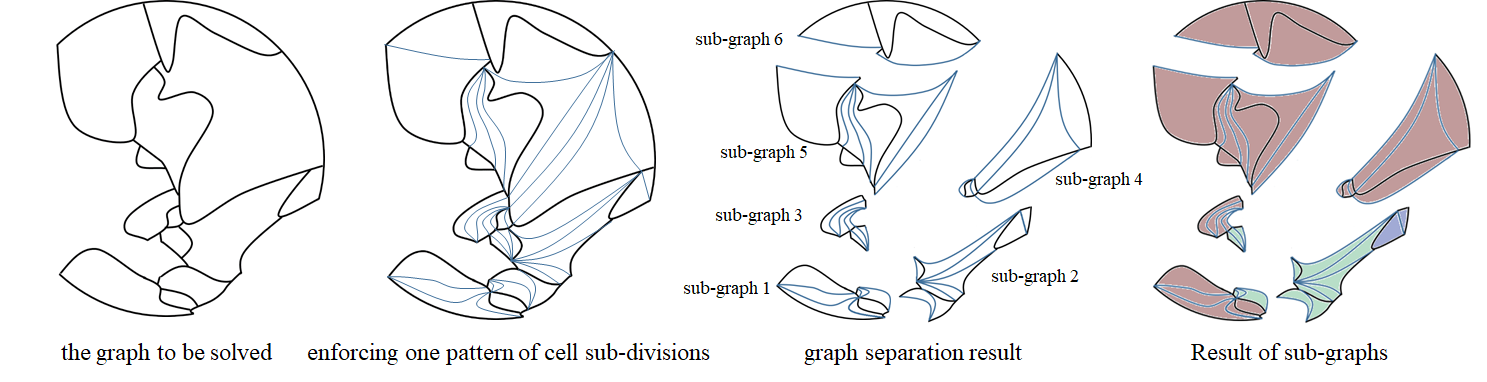
\includegraphics[width =0.96\textwidth]{figures/graph_separation_2}
\caption{Illustration of how an unsolved graph is separated into sub-graphs. }\label{fig:complicated_graph}
\end{figure*}




\subsection{Defining Strips}
\begin{color}{blue}
\begin{proposition}
In a graph enforced that 
\begin{enumerate}
\item Each cell has at most $3$ adjacent cells, and
\item Internal cells are non-adjacent, 
\end{enumerate}
then the graph is an intersection-free graph. 
\end{proposition}
\begin{proof}
It is observed that when a part of the graph contains an intersection, there must exist at least $4$ entries. Moreover, each entry may not be a single edge.  
These motivate us to consider its opposite: if 1) is satisfied, then there can not possibly be an intersection. 
In noting that two internal $3$-edge cells may form a $4$-edge cell which breaks this criterion, 2) is required. 
\end{proof}
With all internal cells being isolated, the graph satisfying the above two constraints is also referred to as a \textit{strip}. 
\end{color}

\subsection{Graph Separation into Strips}
At this point in the start of the separation process it can be safely assumed that all multi-edge cells have been divided. 
Please refer to Fig.~\ref{fig:steps} for a visualisation of the separation process with an example. One boundary cell is first selected and regarded as an element of strip $1$, shown in green in Fig.~\ref{fig:steps}(a).
Then, for each adjacent cell of the strip, we check whether accommodating this cell into the strip will violate the constraints discussed earlier. 
Otherwise it is inserted. 
When no further cells can be inserted, the construction of strip $1$ is deemed finished. 
In this example, as shown in Fig.~\ref{fig:steps}(a), adjacent cells are iteratively inserted to strip $1$ which are shown in blue. If one more cell is inserted, then the boundary cell $5$ (illustrated in detail in Fig.~\ref{fig:characteristic_string}) will become an internal cell which is adjacent to the internal cell $2$, so the construction of strip $1$ terminates.  
To construct strip $2$, we check one-by-one whether the cells adjacent to strip $1$ can be inserted. 
After that, all adjacent cells to strip $2$  are again checked and attempted to be inserted into strip $3$. 
%Then adjacent cells of strip $2$ are iteratively checked to be included. 
By iteratively considering adding the adjacent cells to the previous strip into the current strip and adding more cells satisfying the two constraints, 
the whole graph is finally separated into strips, as shown in Fig.~\ref{fig:complicated_graph} where the example graph is separated into $6$ sub-graphs. (The process corresponds to line \ref{alg:separation_start} $\sim$ line \ref{alg:separation_end} in \textbf{Algorithm} \ref{alg:1}.) 


\begin{algorithm}[t]
    \caption{Improved Solver}\label{alg:1}
    \begin{algorithmic}[1]
        \Require The initial graph $G = (\{C_i\}_{i = 1}^M, \{E_j\}_{j = 1}^N)$  
        \Ensure All solved graphs $\{result\}$  
\For{all $E_1$ ways of divisions of cell $1$} 
\If{non-optimality is detected}
\State \textbf{continue}
\EndIf
\State $\ddots$
	\For{all $E_M$ ways of divisions of cell $M$}
	\If{non-optimality is detected}
	\State \textbf{continue}
	\EndIf
	\State // Graph Separation
		\While{the graph is not intersection-free}\label{alg:separation_start}
		\State Choose a cell to be in the new strip
		\State Attach new cells satisfying constraints
		\State separate the strip from the graph
		\EndWhile\label{alg:separation_end}
		\State // Let there be $n$ strips generated
		\For{all characteristic strings of strip $1$}
		\State $\ddots$
		\For{all characteristic strings of strip $n$}
		\State Combine strips to form a solution $S$\label{alg:combining_start}
		\If{it is better than $\{result\}$}
		\State $\{result\} = \varnothing$
		\State push $S$ into $\{result\}$
		\Else
		\If{it is currently optimal}
			\State push $S$ into $\{result\}$
		\EndIf
		\EndIf\label{alg:combining_end}
		\EndFor
		\State $\udots$
		\EndFor

	\EndFor
\State $\udots$
\EndFor% cell 1 sub-division
    \end{algorithmic}  
\end{algorithm}

\end{color}

\subsection{Solving Strips}
After the graph has been separated, all the solutions for each strip are enumerated via iterating through all the possible characteristic strings. 
Note that there is no extra memory cost for this step - all sub-graph solutions are indexed by the characteristic strings, so they can be randomly accessed 
to be able to pick up any solution of one sub-graph to combine with another sub-graphs, resulting in a given solution to the original graph. 

%\section{Full Graph Solution}\label{section_full_graph}
\begin{color}{blue}
\subsection{Full Graph Solution}
\end{color}
Picking up one solution from each sub-graph, they are combined to form a solution of the original graph. 
The edges identified during the graph separation process are automatically solved by comparing the colour of its two adjacent cells. 
A cost is calculated whose physical meaning is the number of connected regions in the painted part of the (combined) sub-graphs~\cite{Yang2020Cellular}. 
%Compared with seeing strips as two separated sub-graph, when combining them, if the adjacent cells of an edge have the same colour, and the cells have not been connected by previous combining process, then the cost $-1$.  
Once the original graph is re-constructed, the number of connected regions in the solution is fully known. Its optimality can be trivially judged against all possible combinations of sub-graph solutions to reach a set with all the optimal solutions. (line \ref{alg:combining_start} $\sim$ line \ref{alg:combining_end} in \textbf{Algorithm} \ref{alg:1})

\section{Complexity}
\label{section_complexity}
\begin{color}{blue}
The target of this section is to prove the exponential improvement on algorithmic complexity over existing approaches, as claimed in abstract and Section~\ref{section_introduction}. 
As mentioned earlier, cell sub-divisions were undertaken before graph separation to avoid the possible  constraint violation caused by cell sub-divisions in sub-graphs. So the algorithm complexity must also be calculated based on this (i.e.no $\prod E_i$ is multiplied for that segment of the procedure).

\begin{theorem}
Given a topological graph to be solved, assume that it has been properly cell sub-divided before running the enumerative solvers. Let there be $M$ topological cells and $N$ internal edges in the graph. The number of edges for the $i$-th cell is $\alpha_i$, and denote the number of available colours to fill cell $i$ as $K_i$. Then, the proposed graph separation-based algorithm has following number of steps for enumerative solving
\begin{equation}
\prod\limits_{j = 1}^M K_j^{\max\{\alpha_j-2, 1\}}
\end{equation}
Compared to the complexity of the full enumeration solution~\cite{Yang2020Cellular}
\begin{equation}
\prod\limits_{j = 1}^M K_j^{\max\{\alpha_j-2, 1\}}\cdot 2^N
\end{equation}
the proposed graphing scheme represents an exponential improvement in 
the order of $2^N$. 
\end{theorem}
\end{color}

\begin{proof}
%The proposed algorithm has been shown to consist of a number of steps: (1) separating a graph into subgraphs, (2) separating each subgraph into strips, solving each strip individually, and constructing all optimal solutions by combining the individual strip solutions. Finally (3) all individual subgraph solutions can be combined to form the solutions to the original graph. 
\textcolor{blue}{The proposed algorithm has been shown to consist of a number of steps: 
\begin{enumerate}
\item separating a graph into strips, 
\item solving each strip individually, and 
\item constructing all optimal solutions of the original graph by combining the individual strip solutions. 
\end{enumerate}
}
\noindent
The overall complexity can thus be calculated individually for each step. 

1) Separating the graph only requires checking on each cell once, and we only need one valid graph separation, so the complexity of this part is denoted by $\Phi = O(M)$. 

2) The complexity of a single strip can be derived as follows: Let there be $r_i$ boundary cells and $s_i$ internal cells in the strip $i$, 
indexed as $( i_1, \cdots, i_{r_i}, i_{r_i+1}, \cdots, i_{r_i+s_i})$, 
and having $(\alpha_{i_1}, \cdots, \alpha_{i_{r_i}}, \alpha_{i_{r_i+1}}, \cdots, \alpha_{i_{r_i+s_i}})$ edges. 
The number of available colours for each cell can be  written as $(K_{i_1}, \cdots, K_{i_{r_i}}, K_{i_{r_i+1}}, \cdots, K_{i_{r_i+s_i}})$. 
Note that the list of cells form a chain, so that other than the start and end cells, each cell will have two internal edges, one shared with its precedent cell and the 
other shared with its successor. As a 2D topological structure, a cell $j$ in the strip will have at least two internal edges, and at most $(\alpha_{i_j}-2)$ edges are exposed to the boundary of the strip. 
Hence, the complexity $\Psi_i$  of solving strip $i$ will be the multiplication of the algorithmic complexity of all boundary cells 
\begin{equation}
\Psi_i = \prod\limits_{j = 1}^{r_i} K_{i_j}^{\max\{\alpha_{i_j}-2, 1\}}
\end{equation}
where $\max\{\alpha_{i_j}-2, 1\}$ represents the case that multiple edges of the same cell may appear in the strip boundary. 
Since the enumeration of the solutions for different strips is fully independent, the combined complexity is just summed up but not muliplied. 
Considering the notation $M = \sum (r_i+s_i)$, the overall complexity of finding the solutions for a sub-graph is given by
\begin{equation}
\begin{aligned}
\Psi = \sum \Psi_i = & \sum\limits_{i} \left(\prod\limits_{j = 1}^{r_i} K_{i_j}^{\max\{\alpha_{i_j}-2, 1\}}\right)\\
\ll & \sum\limits_{i} \left(\prod\limits_{j = 1}^{r_i+s_i} K_{i_j}^{\max\{\alpha_{i_j}-2, 1\}}\right)\\
\ll&\prod\limits_{i}\left(\prod\limits_{j = 1}^{r_i+s_i} K_{i_j}^{\max\{\alpha_{i_j}-2, 1\}}\right)\\
=&\prod\limits_{j = 1}^M K_j^{\max\{\alpha_j -2, 1\}}
\end{aligned}
\end{equation}

3) For the final step of the algorithm, the complexity is the multiplication of the algorithmic complexity of all sub-graphs 
\begin{equation}
\begin{aligned}
\Xi = \prod \Psi_i = & \prod\limits_i \left(\prod\limits_{j = 1}^{r_i} K_{i_j}^{\max\{\alpha_{i_j}-2, 1\}}\right)\\
\ll&  \prod\limits_i \left(\prod\limits_{j = 1}^{r_i+s_i} K_{i_j}^{\max\{\alpha_{i_j}-2, 1\}}\right)\\
\ll& \prod\limits_{j = 1}^M K_j^{\max\{\alpha_j-2, 1\}}
\end{aligned}
\end{equation}
The overall complexity of the proposed algorithm is the sum of $\Phi$, $\Psi$ and $\Xi$, 
\begin{equation}
\Gamma =\Phi+\Psi+\Xi \ll  \prod\limits_{j = 1}^M K_j^{\max\{\alpha_j-2, 1\}}
\end{equation}
\end{proof}

\begin{comment}
Compared to the complexity of the full enumeration solution~\cite{Yang2020Cellular}
\begin{equation}
\prod\limits_{j = 1}^M K_j^{\max\{\alpha_j-2, 1\}}\cdot 2^N
\end{equation}

It can be observed how the proposed graphing scheme represents an exponential improvement in 
the order of $2^N$, with $N$ being the number of topological edges in the graph. 
\end{comment}

%\begin{figure*}[t]
%\centering
%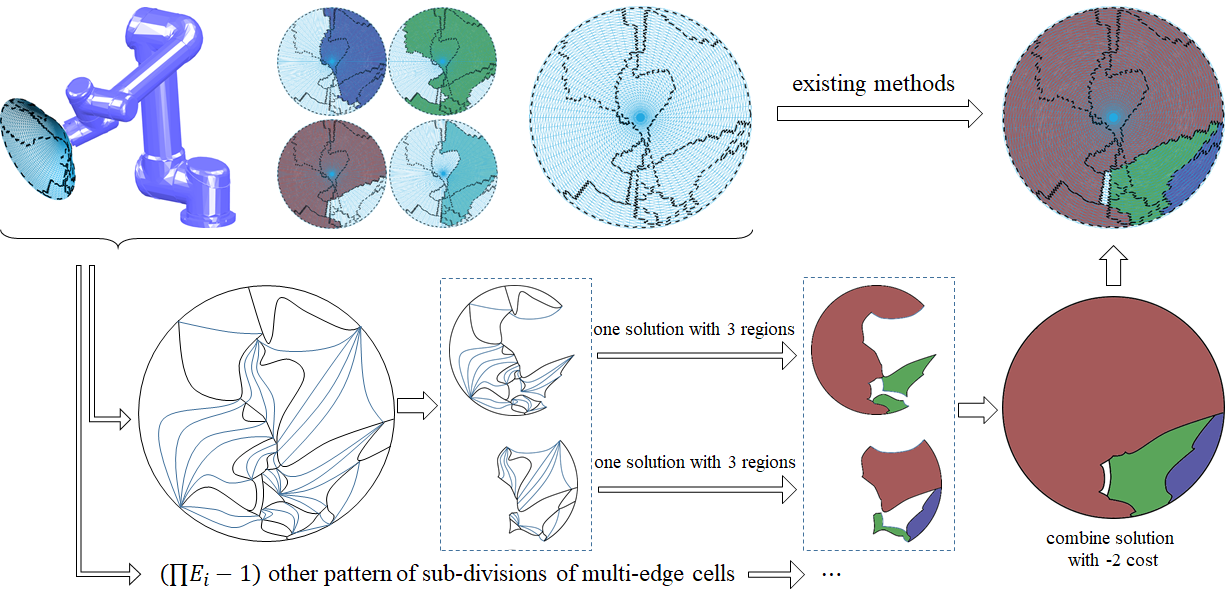
\includegraphics[width = 0.96\textwidth]{figures/hat_exp/fig_hat}
%\caption{\textcolor{blue}{What if I directly use the sub-graph in this experiment to be the demo figures of the above algorithm section? }}\label{fig:hat}
%\end{figure*}

\begin{figure}[t]
\centering
\subfigure[]{
	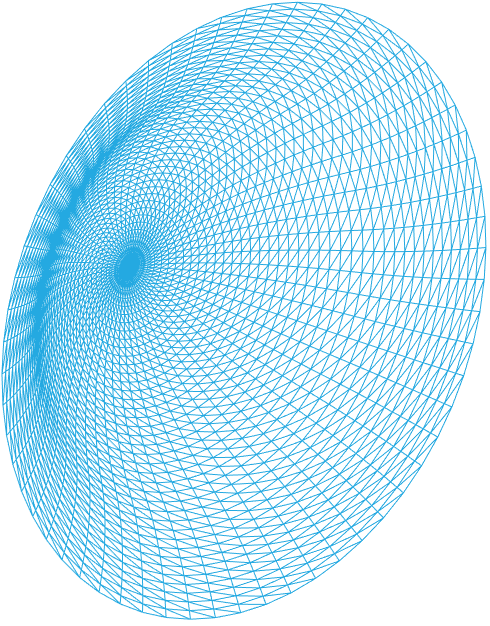
\includegraphics[width=0.15\textwidth]{figures/hat_exp/mesh}
}
\subfigure[]{
	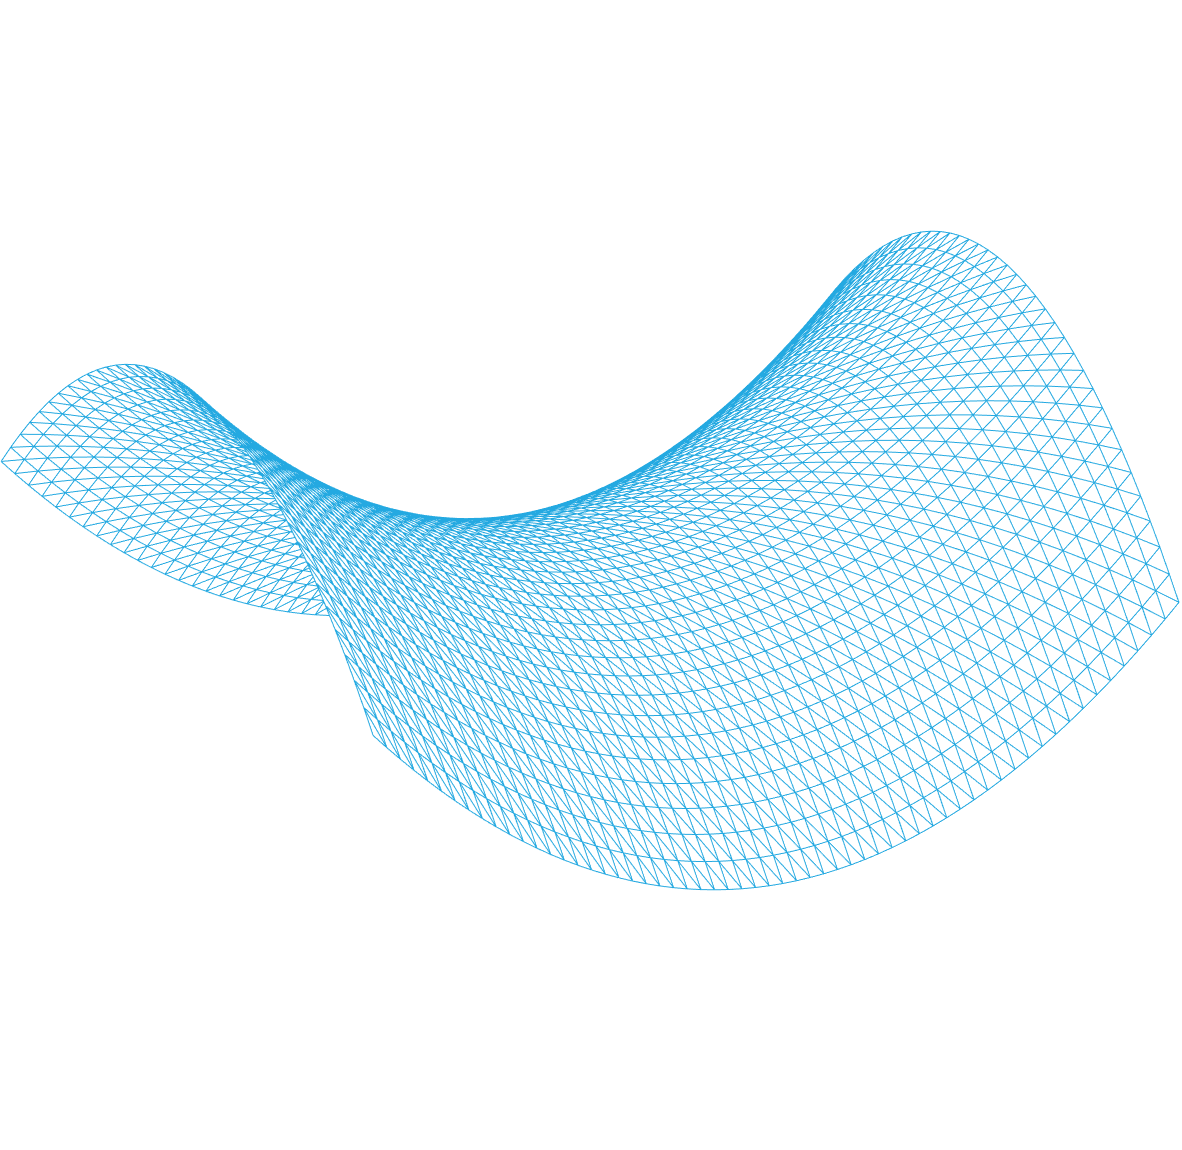
\includegraphics[width=0.15\textwidth]{figures/saddle_exp/mesh}
}
\caption{The objects used for illustration in Section \ref{section_results}. }\label{fig:object}
\end{figure}

\begin{figure*}[t]
\centering
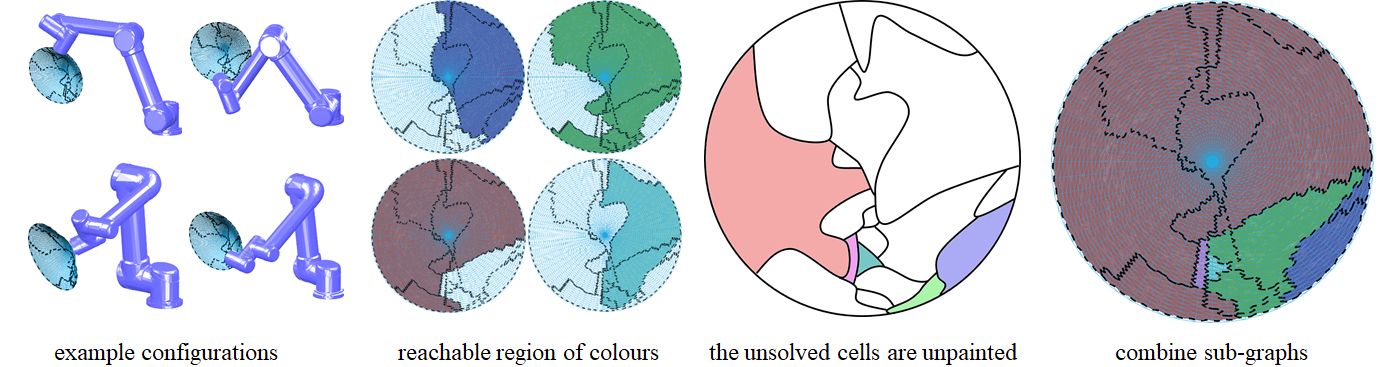
\includegraphics[width=0.96\textwidth]{figures/hat_exp/fig_hat_2}
\caption{The coverage task on a hat-shape object. The reachable area of different colours and one of their corresponding configurations are depicted. After painting all $1$-colour cells, the unsolved graph is exactly the same one as we have discussed in Section \ref{section_graph_separation}. }\label{fig:hat}
\end{figure*}
\begin{figure*}[t]
\centering
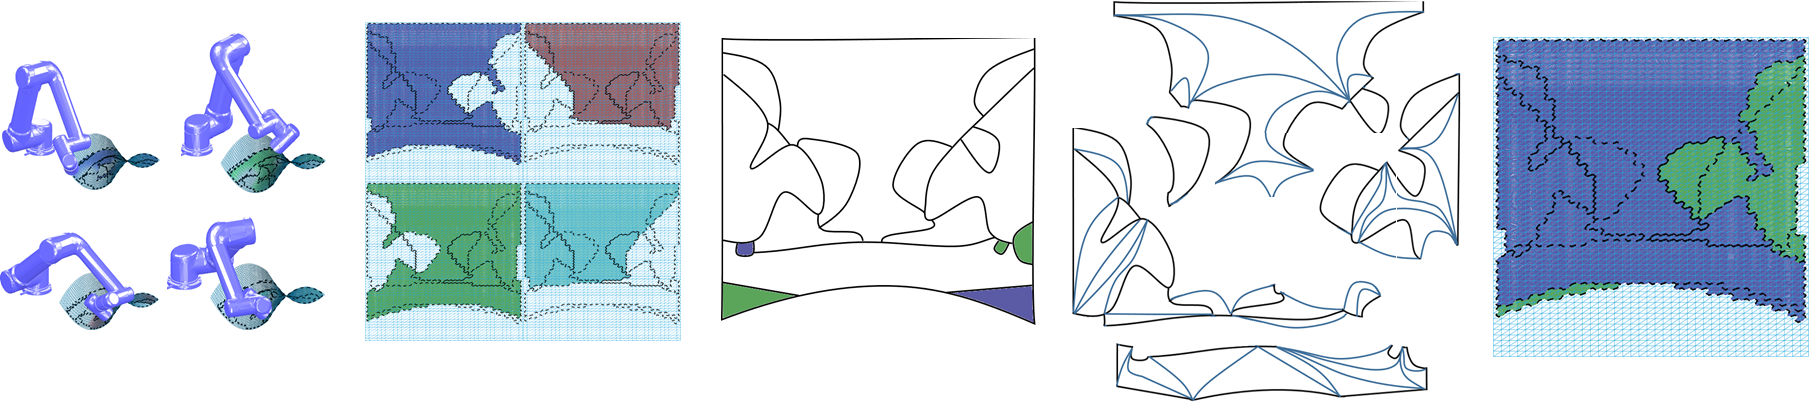
\includegraphics[width=0.96\textwidth]{figures/saddle_exp/comb}
\caption{The coverage task on a saddle surface. The reachable area of different colour and one of their corresponding configurations are depicted. After painting all $1$-colour cells, the unsolved grpah is separated into $5$ sub-graphs. Finally, all optimal solutions can be collected with 2 end-effector lift-offs.    }
\label{fig:saddle}
\end{figure*}

\section{Experimental Results}\label{section_experiment}
\label{section_results}

The proposed solution is tested experimentally by simulating the NCPP with a non-redundant manipulator (6 DoF Universal Robot UR5) on two arbitrarily shaped objects, one a hat-like concave semi-sphere (only one side is considered), and a saddle surface (only one side being considered also), as shown in Fig.~\ref{fig:object}.

\subsection{Optimal NCPP on a Hat-shape Object}
% <ty> Suddenly I notice that the demo figure is not illustrative. Will change
An illustration of the solving process for the hat-shape object is depicted in Fig.~\ref{fig:hat}. 
Four continuous sets of manipulator configurations are represented in blue, red, green and cyan colour separately. $1$-colour cells have been directly drawn to the graph. 
%Using existing algorithms~\cite{Yang2020Cellular}, the initial topological graph is directly enumerated. We need to iteratively decide whether keep/remove each topological edges, and choose colour for each (sub-)cells, leading to complexity as (\ref{equ:tmech}). One of the graph after cell sub-divisions is shown in Fig.~\ref{fig:hat}.  
The cell sub-divisions correspond to the description provided earlier in Fig.~\ref{fig:complicated_graph}.
For the algorithmic complexity there are $43$ cells. The possible colours of each cell are known. As for edges, there are $44$ unsolved edges (drawn in black) and $30$ manually created edges - enforced to be kept (drawn in blue). Plus $9$ edges which are connected to unreachable area (a fifth colour), which need not solving. Using the naive enumeration proposed in the literature, %~\cite{Yang2020Cellular} - we've repeated this too many times I feel
$35$ edges and all colours of all cells are enumerated, resulting in an algorithmic complexity described by 
\begin{equation}
{\color{red}2^{35}\times}
\begin{aligned}
&\overbrace{2\times2\times3\times2\times2\times2\times{\color{red}2\times2\times}}^{\textbf{all cells in sub-graph 1, shown in Fig.~\ref{fig:characteristic_string}}}\\
&2\times3\times3\times2\times2\times3\times2\times3\times2\times{\color{red}3\times}\\
&2\times2\times2\times2\times2\times2\times{\color{red}2\times}\\
&2\times3\times3\times4\times4\times{\color{red}3\times4\times}\\
&3\times3\times2\times3\times3\times4\times4\times{\color{red}3\times}\\
&3\times4\times3
\end{aligned}
\approx 1.2705\times10^{28}
\end{equation}
Please note there is a minor abuse of notation in the arrangement of the numbers above simply so that they can be easier to compared with the optimal solution below. 
%\begin{equation}
%2^{35}\cdot \underbrace{2\times 2\times \cdots \times 3}_{43 \mbox{ terms, number of colours}} \approx 1.2705*10^{28}
%\end{equation}

Using the proposed algorithm, the length of the boundary for each sub-graph is $6, 11, 9, 6, 10, 5$ respectively. The reader is referred to the sub-graph $1$ example
employed to discuss the process in detail in Sections~\ref{section_intersection} and~\ref{section_graph_separation}. Detail results for the others cases are ommited for lack of space, 
but follow the same process. 
The number of colours for the boundary cells in each sub-graph is included in the multiplicative factor, so the algorithm complexity derives in the multiplication of 
the complexity of all sub-graphs, given by 
\begin{equation}
\begin{aligned}
&\overbrace{2\times2\times3\times2\times2\times2\times}^{\textbf{internal cells shown in Fig.\ref{fig:characteristic_string}}}\\
&2\times3\times3\times2\times2\times3\times2\times3\times2\times\\
&2\times2\times2\times2\times2\times2\times\\
&2\times3\times3\times4\times4\times\\
&3\times3\times2\times3\times3\times4\times4\times\\
&3\times4\times3
\end{aligned} \approx 4.2797\times10^{14}
\end{equation}

\subsection{Optimal NCPP on a Saddle-shape Object}
Another example is provided with the analysis of the outer shell of a saddle-shape object. In this case the surface normal varies greatly as the end-effector moves 
along the surface, representing a challeging manipulator planning problem in adopting poses that would benefit the continuous coverage this paper is interested in. 
The algorithmic complexity given cell sub-divisions is shown in Fig.~\ref{fig:saddle}. For the  naive enumeration case, the overall complexity is given by 
%\begin{equation}
\begin{flalign}
&{\color{red}2^{47}*}~
\begin{aligned}
&2\times2\times2\times2\times2\times2\times2\times2\times2\times{\color{red}2\times}\\
&3\times2\times2\times2\times2\times2\times2\times \\
&~~~~3\times4\times4\times3\times2\times2\times2\times3\times{\color{red}3\times}\\
&3\times2\times2\times2\times2\times3\times3\times2\times{\color{red}2\times}\\
&4\times4\times4\times4\times4\times4\times3\times4\times{\color{red}4\times}\\
&3
\end{aligned}&\\
&\approx 2.924\times10^{32}&\nonumber
\end{flalign}
%\end{equation}
Applying the proposed algorithm, the complexity is reduced to
\begin{flalign}
&\begin{aligned}
&2\times2\times2\times2\times2\times2\times2\times2\times2\times\\
&3\times2\times2\times2\times2\times2\times2\times\\
&~~~~3\times4\times4\times3\times2\times2\times2\times3\times\\
&3\times2\times2\times2\times2\times3\times3\times2\times\\
&4\times4\times4\times4\times4\times4\times3\times4\times\\
&3
\end{aligned}
\approx 4.3283\times10^{16}&
\end{flalign}
The overall results are gathered in Table~\ref{table:results} for easier comparison, collecting the substantial computational improvement in 
the number of edges for each problem ($35$ and $47$ repectively). As the geometry of the object of interest becomes more intricate, 
the benefit of the proposed scheme to be able to find paths with minimal discontinuities in joint-space with a reduced computational effort 
becomes also more apparent.
\begin{table}
\centering
\caption{Experimental results}
\begin{tabular}{ | c | c | c | c | c | }
 \hline
  \multirow{2}{*}{Object}  & \multicolumn{2}{|c|}{Number of Iterations} \\
\cline{2-3}
  						& Full enumeration~\cite{Yang2020Cellular}  &  Proposed Optimal \\
 \hline
 Hat-shaped (Fig.~\ref{fig:hat})   	& $1.2705*10^{28}$    				&   $4.2797*10^{14}$\\
 \hline
 Saddle-shaped (Fig.~\ref{fig:saddle})					&   $2.924*10^{32}$  		&   	$4.3283*10^{16}$\\
 \hline
\end{tabular}
\label{table:results}
\end{table}


%\begin{table}
%\begin{tabular}{ | c || c | c | c | c | }
% \hline
%  Object  & \multicolumn{4}{|c|}{Solver} \\
% \hline
%  						& \multicolumn{2}{|c|}{Full enumeration~\cite{Yang2020Cellular}}  &  \multicolumn{2}{|c|}{Proposed Optimal} \\
% \hline
% 						&  $\Gamma$  & time(sec.)? other to compare? 	& $\Gamma$ & time?\\
% \hline
% Hat-shaped ( Fig.~\ref{fig:hat})   	& X    		& Y		&   X' 		& Y'\\
% \hline
% Other (Fig.~\ref{fig:saddle})					&  a  		& b   		& a'   		& b'\\
% \hline
%\end{tabular}
%\caption{Experimental results. Computational time calculated on a Pentium ... configuration machine.}
%\end{table}


\begin{comment}
Several representative simulation works have been implemented to validate the proposed algorithm on challenging  arbitrarily-shaped objects.
% the optimal non-revisiting coverage planning path is solved. 
Fig. \ref{fig_mobius_exp} presents the solution of polishing a Mobi\"{u}s strip, whose surface is non-orientable. The manipulator is required to maintain the EE normal to the surface for proper operation simulating a contact task such as polishing. This is rather challenging in this case 
since the strip is twisted, hence the orientation of the normal vector varies over the full $2\pi$ rads. However, the proposed algorithm 
is able to come up with a configuration mapping leading to an optimal solution where only $1$ lift-off is required over the entire object.

Fig. \ref{fig_ring_exp} depicts the process of covering the surface of a ``swimming'' ring, another closed surface with no boundary. 
This is a particularly challenging case, it can be seen how the topological graph is formed by cells that are all multiply-connected, 
yet the proposed algorithm is able to come up with an effective solution with a single configuration discontinuity to the NCPP problem. 

The examples in Fig.~\ref{fig:hill_multiply_conn}, Fig.~\ref{fig_hill_exp_0_10} and Fig.~\ref{fig_hill_exp_0_16} illustrate the solutions of covering a ``hilly terrain" with varying degrees of desirable manipulability~\cite{Yoshikawa1990Translational}. 
For a given configuration (colour) cell, the manipulability is explicitly depicted brighter for increasing manipulability for the given configuration. The threshold  varies from a minium of $0.06$ (Fig.~\ref{fig:hill_multiply_conn}) to at least $0.10$ (Fig.~\ref{fig_hill_exp_0_10}), up to at least $0.16$, the maximum where a solution can be found for the object (in Fig.~\ref{fig_hill_exp_0_16}).
As one would expect, a sharp reduction in the reachable area is observed as the manipulability tightens 
(mainly due to the limited mobility of the wrist-flipped configurations, shown in the bottom two configurations 
in Fig.~\ref{fig:manip_010_configs}), causing large fluctuations in the structure of the resulting cells and topology graphs. When the threshold goes to $0.16$, most of the kinematic-valid wrist-unflipped configurations are no longer valid, as depicted in Fig.~\ref{fig_hill_exp_0_16}. 
\end{comment}

\section{Conclusions}
An advancement to efficiently solve non-repetitive coverage tasks with a non-redundant manipulator is proposed in this work. 
The core concept is the introduction of topological intersections and intersection-free graphs, which permit the separation of a graph 
into sub-graphs at the points where the multiplicity of optimal solutions originate. 
The implicit enumeration of these intersections when the graphs are recombined in search of the full solution derive in a mathematically proven exponential improvement in the order of $2^N$, $N$ representing the number of topological edges in the graph. This is particularly relevant for intricate task-space graphs,
where an exhaustive search for solutions with all the cells and edges is unattainable. 
Comprehensive experimental results with step-by-step derivations to illustrate the proposed algorithm are supplied that demonstrate the validity of the novel scheme. 
\label{section_conclusion}


%% Use plainnat to work nicely with natbib. 

%\newpage 

\bibliographystyle{ieeetr}
\bibliography{improved_solver}

\end{document}


